\let\counterwithout\relax
\let\counterwithin\relax
\documentclass[final]{fhnwreport}       %[mode] = draft or final
\usepackage{color, colortbl}
                                        %{class} = fhnwreport, article, 
                                        %          report, book, beamer, standalone
%%---Main Packages-----------------------------------------------------------------------
\usepackage[english, ngerman]{babel}	%Mul­tilin­gual sup­port for LaTeX
\usepackage[T1]{fontenc}				%Stan­dard pack­age for se­lect­ing font en­cod­ings
\usepackage[utf8]{inputenc}				%Ac­cept dif­fer­ent in­put en­cod­ings
\usepackage{lmodern}                    %The newer Font-Set
\usepackage{textcomp}					%LaTeX sup­port for the Text Com­pan­ion fonts
\usepackage{graphicx} 					%En­hanced sup­port for graph­ics
\usepackage{float}						%Im­proved in­ter­face for float­ing ob­jects
\usepackage{ifdraft}                    %Let you check if the doc is in draft mode

%%---Useful Packages---------------------------------------------------------------------
\usepackage[pdftex,dvipsnames]{xcolor}  %Driver-in­de­pen­dent color ex­ten­sions for LaTeX
\usepackage{csquotes}                   %Simpler quoting with \enquote{}
\usepackage{siunitx} 					%A com­pre­hen­sive (SI) units pack­age
\usepackage{listings}					%Type­set source code list­ings us­ing LaTeX
\usepackage[bottom]{footmisc}			%A range of foot­note op­tions
\usepackage{footnote}					%Im­prove on LaTeX's foot­note han­dling
\usepackage{verbatim}					%Reim­ple­men­ta­tion of and ex­ten­sions to LaTeX ver­ba­tim
\usepackage[textsize=footnotesize]{todonotes} %Mark­ing things to do in a LaTeX doc­u­ment

%%---Tikz Packages-----------------------------------------------------------------------
\usepackage{standalone}
\usepackage{tikz}
\usepackage{circuitikz}
\usetikzlibrary{arrows}
\usetikzlibrary{calc}
\usetikzlibrary{intersections}

%%---Math Packages-----------------------------------------------------------------------
\usepackage{amsmath}					%AMS math­e­mat­i­cal fa­cil­i­ties for LaTeX
%\usepackage{amssymb}					%Type­set­ting symbols (AMS style)
%\usepackage{array}						%Ex­tend­ing the ar­ray and tab­u­lar en­vi­ron­ments
%\usepackage{amsthm}					%Type­set­ting the­o­rems (AMS style)

%%---Table Packages----------------------------------------------------------------------
\usepackage{tabularx}					%Tab­u­lars with ad­justable-width columns
%\usepackage{longtable}
\usepackage{multirow}					%Create tab­u­lar cells span­ning mul­ti­ple rows
\usepackage{multicol}					%In­ter­mix sin­gle and mul­ti­ple columns

%%---PDF / Figure Packages---------------------------------------------------------------
\usepackage{pdfpages}					%In­clude PDF doc­u­ments in LaTeX
\usepackage{pdflscape}					%Make land­scape pages dis­play as land­scape
\usepackage{subfig}					    %Fig­ures di­vided into sub­fig­ures

%%---Other Packages----------------------------------------------------------------------
%\usepackage{xargs}                     %De­fine com­mands with many op­tional ar­gu­ments

%%---Bibliography------------------------------------------------------------------------
\usepackage[style=ieee,urldate=comp,backend=biber, natbib=true]{biblatex}
\addbibresource{literature/bibliography.bib}

%%---Main Settings-----------------------------------------------------------------------
\graphicspath{{./graphics/}}			%Defines the graphicspath
%\geometry{twoside=false}				    %twoside=false disables the "bookstyle"
\setlength{\marginparwidth}{2cm}
\overfullrule=5em						%Creates a black rule if text goes over the margins => debugging


%%---User Definitions--------------------------------------------------------------------
%%Tabel-Definitions: (requires \usepackage{tabularx})
\newcolumntype{L}[1]{>{\raggedright\arraybackslash}p{#1}}    %column-width and alignment
\newcolumntype{C}[1]{>{\centering\arraybackslash}p{#1}}
\newcolumntype{R}[1]{>{\raggedleft\arraybackslash}p{#1}}

%%---Optional Package Settings-----------------------------------------------------------
%Listings-Settings: (requires \usepackage{listings}) => Example with Matlab Code
\lstset{language=Matlab,%
    basicstyle=\footnotesize\ttfamily,
    breaklines=false,%
    morekeywords={switch, case, otherwise},
    keywordstyle=\color{Blue},%
    tabsize=2,
    %morekeywords=[2]{1}, keywordstyle=[2]{\color{black}},
    identifierstyle=\color{Black},%
    stringstyle=\color{Purple},
    commentstyle=\color{Green},%
    showstringspaces=false,%without this there will be a symbol in the places where there is a space
    numbers=left,%
    numberstyle={\tiny \color{black}},% size of the numbers
    numbersep=9pt, % this defines how far the numbers are from the text
    %emph=[1]{word1, word2,...},emphstyle=[1]\color{red}
}							
			                %loads all packages, definitions and settings												
\title{Kleinwasserkraftwerk}          %Project Title
\author{Pflichtenheft}          %Document Type => Technical Report, ...
\date{Windisch, 05.10.2018}             %Place and Date

\begin{document}

%%---TITLEPAGE---------------------------------------------------------------------------
\selectlanguage{ngerman}                %ngerman or english
\maketitle

\vspace*{-1cm}						    %compensates the space after the date line.
\vfill
\begin{figure}[H]
\centering

\includegraphics[width=\linewidth]{titelBild.jpg}
\end{figure}
\vfill

{
\renewcommand\arraystretch{2}
\begin{center}
\begin{tabular}{ >{\bf} l p{10cm} l }
Hochschule&Hochschule für Technik - FHNW\\
Studiengang&Elektro- und Informationstechnik\\
Autoren&Gruppe 4\\%Bachmann Lars \newline  Fischer Roni \newline Imhof Frank \newline Puschmann Pascal\\ 
Betreuer&Pascal Buchschacher\\
Auftraggeber&Felix Jenni\\
Version&1.0 %Normally not used!
\end{tabular}
\end{center}
}

\clearpage

\selectlanguage{ngerman}				%ngerman or english
\thispagestyle{empty}
			
%%---TABLE OF CONTENTS-------------------------------------------------------------------
\pagenumbering{Roman}		
\selectlanguage{ngerman}				%ngerman or english
\tableofcontents
\clearpage

%%---TEXT--------------------------------------------------------------------------------
\pagenumbering{arabic}
\section{Einleitung}

Weltweit wachsen Städte immer mehr in die Höhe. Um in hohen Gebäuden Trinkwasser in die oberen Stockwerke zu pumpen, wird viel Energie benötigt. Das entstehende Abwasser hat eine dementsprechend hohe potentielle Energie, die ungenutzt bleibt, wenn das Wasser zurück in die Kanalisation fliesst. Zudem muss das Wasser bei grosser Fallhöhe noch abgebremst werden, bevor es zurück in die Kanalisation geleitet werden kann. Dabei geht die Energie in Form von Wärme verloren. 

Um Energie zurück zu gewinnen, soll das Abwasser durch eine Turbine geführt werden, die einen Generator antreibt. Damit kann der Strom zurück zu den Wasserpumpen geführt werden, die frisches Trinkwasser in die oberen Stockwerke pumpen. Alternativ kann der Strom auch in das Stromnetz zurückgespeist werden. 

Im Rahmen des Pro1E wollen wir ein solches Abwasser - Kleinkraftwerk unter den Aspekten der Machbarkeit, Wirtschaftlichkeit und des Umweltschutzes untersuchen.  

Die Studierenden werden im Projekt 1 (pro1E) für den Studiengang Elektro- und Informatitonstechnik von drei Dozenten der Fachhochschule Nordwestschweiz (FHNW) unterstützt. Pascal Buchschacher informiert über Projektmanagement allgemein, Anita Gertiser vermittelt den Studenten die richtige Kommunikation innerhalb des Teams und Felix Jenni steht als Ansprechpartner für Fragen technischer Natur zur Verfügung.






\section{Projektorganisation}

Die Studierenden werden im Projekt 1 (pro1E) für den Studiengang Elektro- und Informati- onstechnik von drei Dozenten der Fachhochschule Nordwestschweiz (FHNW) unterstützt. Pascal Buchschacher informiert über Projektmanagement allgemein, Anita Gertiser vermit- telt den Studenten die richtige Kommunikation innerhalb des Teams und Felix Jenni steht als Ansprechpartner für Fragen technischer Natur zur Verfügung.

Dieser Teil des Pflichtenhefts wurde erstellt, um den organisatorischen Teil des Projekt 1 abzudecken. Er zeigt die allgemeine Projektorganisation, die Planung, das Budget und die Risikoanalyse auf.
\subsection{Projektverantwortliche}

\subsection{Auftraggeber}
Auftraggeber des Projekts 1 ist Jenni Felix, Dozent an der Fachhochschule Nordwestschweiz.

\subsection{Teammitglieder}
Das Team 3 des Projekts 1, setzt sich aus sechs Studenten der Fachhochschule Nordwestschweiz, Hochschule für Technik in Brugg/Windisch zusammen. Frank Imhof ist der Projektleiter und verantwortlich für die Arbeiten und die Kommunikation mit dem Auftraggeber und den Fachdozenten. Unterstützt wird dieser vom stellvertretenden Projektleiter Pascal Puschmann. Die übrigen Mitglieder sind Michel Alt, Lars Bachmann,Roni Fischer und Christoph Kuhn. Jeder von ihnen studiert Elektro- und Informationstechnik im ersten Semester, mit Ausnahme von Christoph Kuhn, der gleichzeitig das Projekt 3 absolviert.

\subsection{Organigramm}
\begin{figure}[H]
	\centering
	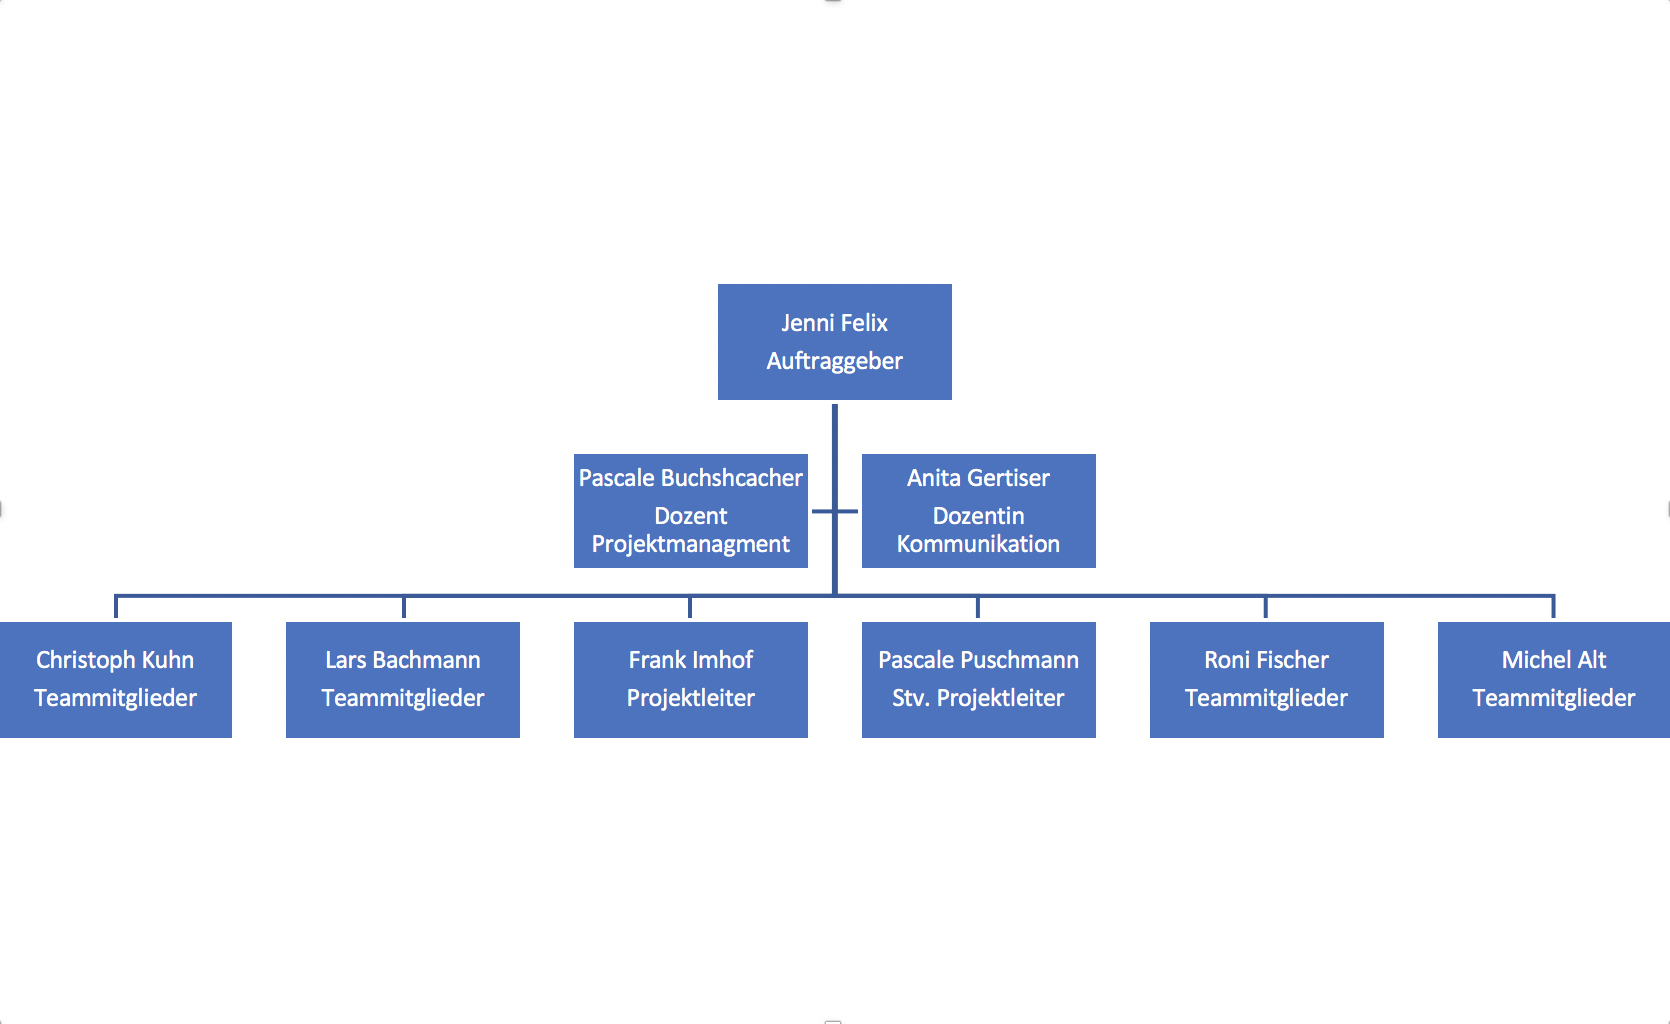
\includegraphics[width=10cm]{organigramm.png}
	\label{fig:Organigramm}
\end{figure}

\section{Projektplanung}
\subsection{Projektablauf-Beschreibung}

\subsection{Projektphasen/Arbeitspakete}
\subsubsection{Projektphasen}

\subsubsection{Arbeitspakete}

\subsubsection{Arbeitspaketgruppen}
\subsection{Projektplan}
\subsubsection{Projektablaufplan}

\subsubsection{Projektzeitplan}

\subsubsection{Ressourcenplan}

\renewcommand{\arraystretch}{1.2}
\definecolor{grau}{gray}{0.9}
\definecolor{hellgrau}{gray}{0.95}
\section{Projektbudget}
\subsection{Personalaufwand}
Für das Erstellen des Budgets wurden folgende Salär-Ansätze verwendet: 
\begin{table}[H]
\begin{tabular}{ll}
Projektleiter:      & 148 CHF/h (nur für Phase Projektmanagement) \\
Projektmitarbeiter: & 74 CHF/h                                   
\end{tabular}
\end{table}

%% Please add the following required packages to your document preamble:
% \usepackage[table,xcdraw]{xcolor}
% If you use beamer only pass "xcolor=table" option, i.e. \documentclass[xcolor=table]{beamer}
\begin{table}[H]
\begin{tabular}{|l|r|r|r|r|}
\hline
\rowcolor[HTML]{C0C0C0} 
Phase                & \multicolumn{1}{l|}{\cellcolor[HTML]{C0C0C0}Stunden} & \multicolumn{1}{l|}{\cellcolor[HTML]{C0C0C0}Stundenanteil} & \multicolumn{1}{l|}{\cellcolor[HTML]{C0C0C0}Kosten} & \multicolumn{1}{l|}{\cellcolor[HTML]{C0C0C0}Kostenanteil} \\ \hline
1. Analyse           & 105 & 23.2\%  &  CHF 7'770.00  & 21.9\%  \\ \hline
2. Entwurf           & 35  &  7.7\%  &  CHF 2'590.00  &  7.3\%  \\ \hline
3. Projektmanagement & 27  &    6\%  &  CHF 3'996.00  & 11.3\%  \\ \hline
4. Dokumentation     & 86  &   19\%  &  CHF 6'364.00  & 17.9\%  \\ \hline
5. Sitzungen         & 160 & 35.3\%  & CHF 11'840.00  & 33.3\%  \\ \hline
6. Reserve           & 40  &  8.8\%  &  CHF 2'960.00  &  8.3\%  \\ \hline
\rowcolor[HTML]{EFEFEF} 
TOTAL                & 453 &  100\%  &  CHF 23'680.0  & 100\%   \\ \hline
\end{tabular}
\end{table}

\begin{table}[H]
\begin{tabular}{ll}
Gesamtkosten: 	 		& CHF 35'520.00 \\
Total Stunden:			& 453			\\
Anzahl Teammitglieder:	& 6				\\
Stunden pro Person: 	& 75.50			                              
\end{tabular}
\end{table}




\section{Risikoanalyse}
\begin{figure}[H]
	\centering
	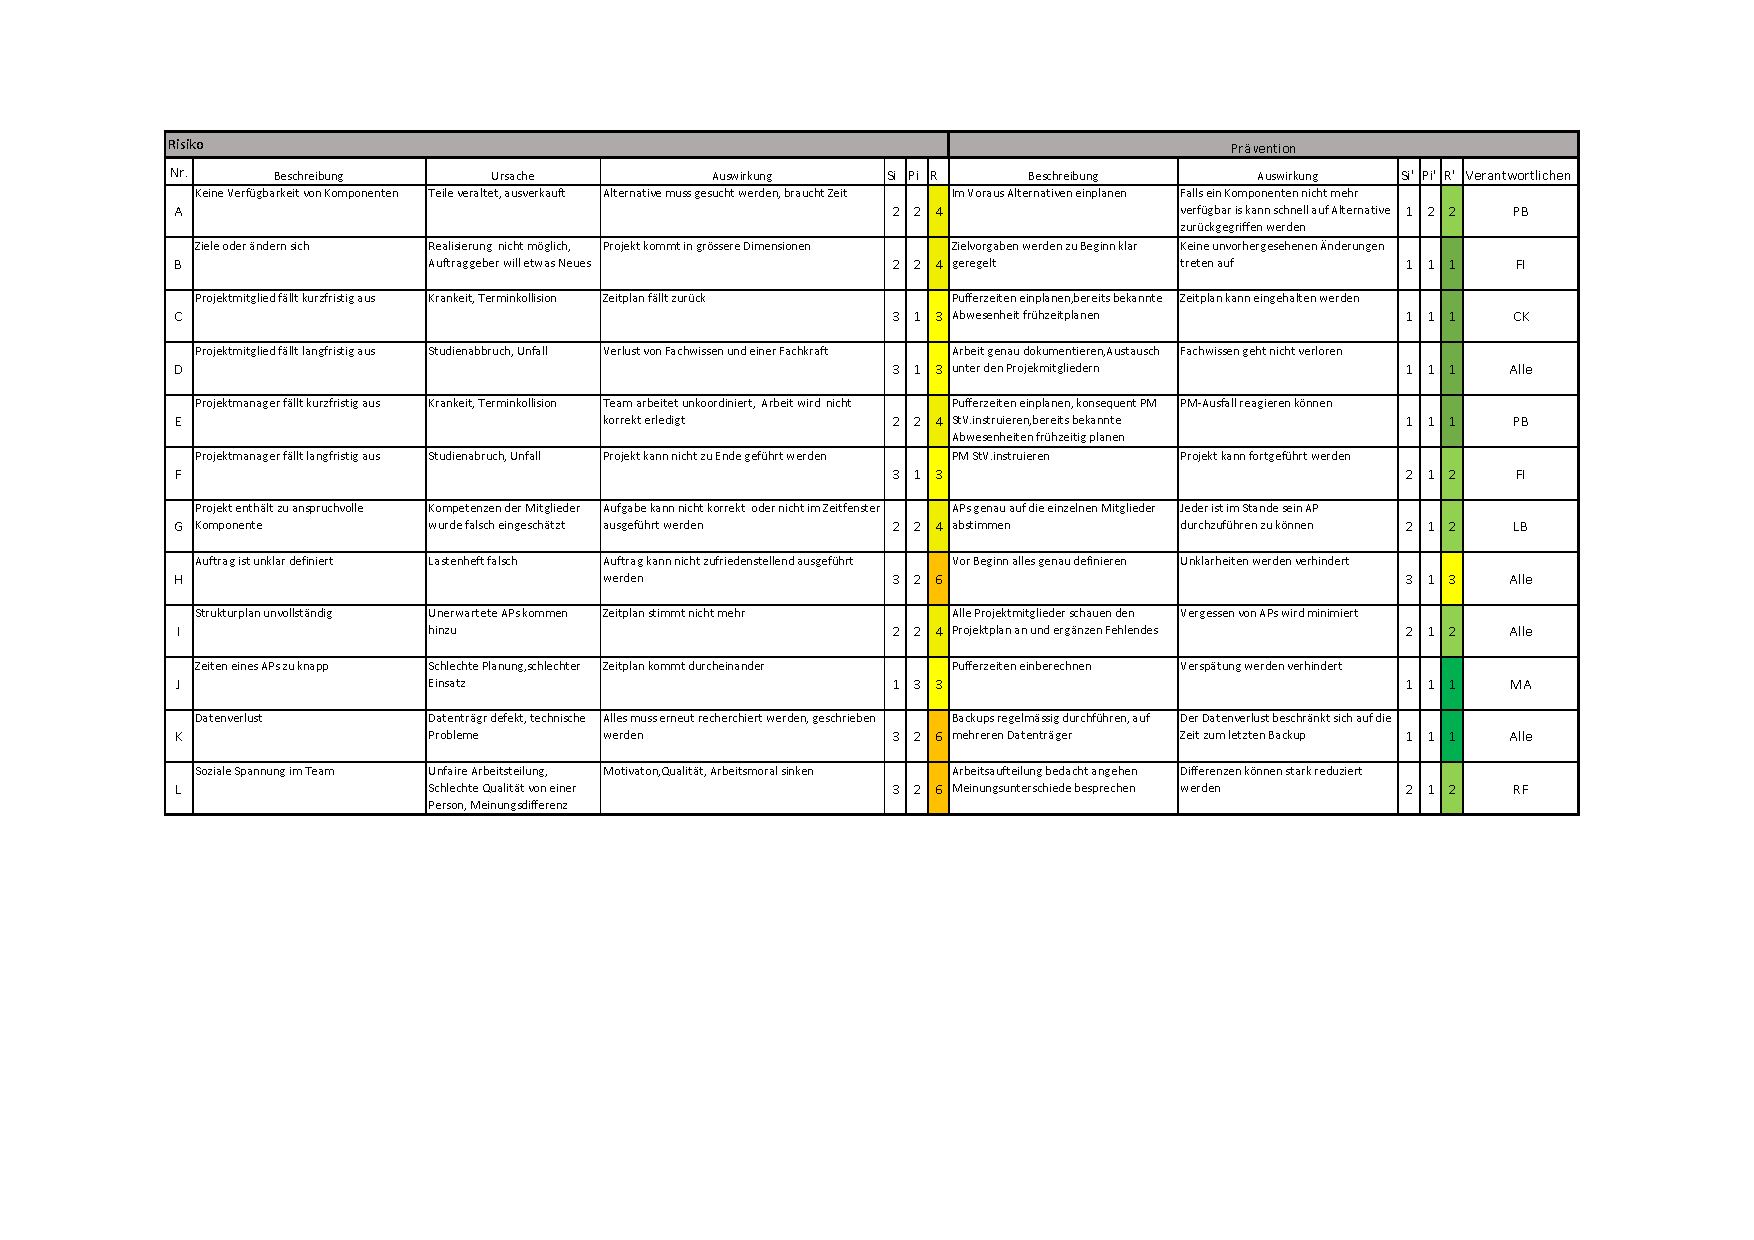
\includegraphics[width=10cm]{Risikoanalyse.pdf}
	\label{fig:Risikoanalyse}
\end{figure}

\newpage

Um auf Risiken vorbereitet zu sein, macht man eine Risikotabelle. In dieser werden die möglichen Ge- fahren aufgelistet und bereits Präventionsmassnahmen genannt, um sowohl die Eintrittswahrscheinlich- keit(Pi), als auch die Auswirkungen(Si) zu minimieren. Auf der Risikomap werden zudem alle Gefahren mit und ohne Prävention graphisch dargestellt.

\begin{figure}[H]
	\centering
	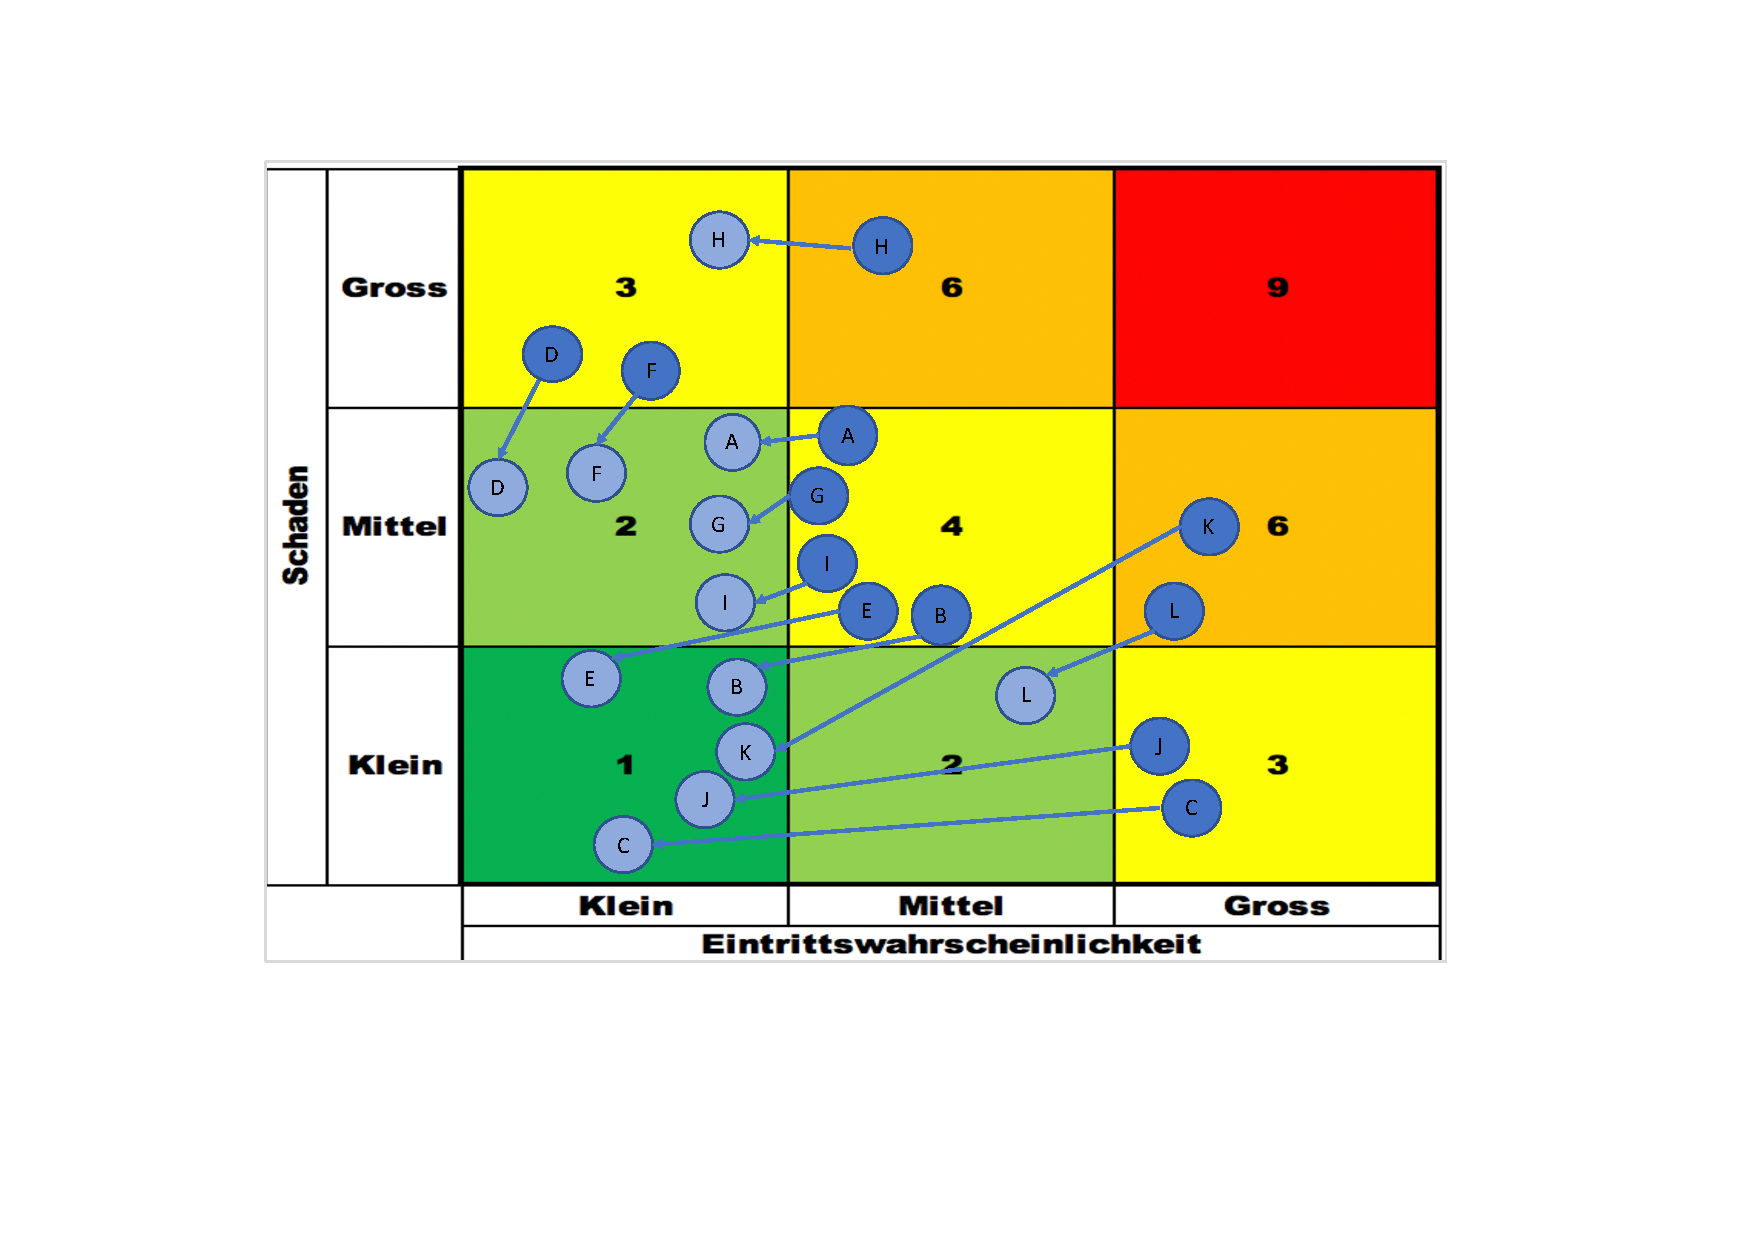
\includegraphics[width=10cm]{Risikotab.pdf}
	\label{fig:Risikodiagramm}
\end{figure}

\begin{figure}[H]
	\centering
	\includegraphics[width=10cm]{si_tabelle}
	\label{fig:Tabelle}
\end{figure}
A Keine Verfügbarkeit von Komponenten
B Ziele ändern sich
C Projektmitglied fällt kurzfristig aus
D Projektmitglied fällt langfristig aus
E Projektmanager fällt kurzfristig aus
F Projektmanager fällt langfristig aus
G Projekt enthält zu anspruchvolle Komponente
H Auftrag ist unklar definiert
I Strukturplan unvollständig
J Zeiten eines APs zu knapp
K Datenverlust
L Soziale Spannung im Team

\section{Projektvereinbarung}
\textbf{Auftraggeber}
Jenni, Prof. Dr. Felix
\bigskip
\hrule
Ort, Datum
\bigskip
\hrule
Ort, Datum


%%---BIBLIOGRAPHY------------------------------------------------------------------------

{\sloppypar
\selectlanguage{english}	
\setlength{\bibitemsep}{\baselineskip}
\printbibliography[heading=bibintoc]
\label{sec:lit}
}

%%---NOTES for DEBUG---------------------------------------------------------------------
\ifdraft{%Do this only if mode=draft
%%requires \usepackage{todonotes})
\newpage
\listoftodos[\section{Todo-Notes}]
\clearpage
}
{%Do this only if mode=final
}
uend{document}
